\chapter{Resultados de Análisis Eléctricos}

\section{Flujos de Carga en Operación Normal}

Los análisis de flujo de carga se realizaron en condición normal de operación, con el fin de evaluar el desempeño del sistema ante la entrada en operación del proyecto fotovoltaico.

\subsection{Análisis de Tensiones}

La entrada en operación del proyecto ocasiona variaciones de tensión en los nodos cercanos al punto de conexión, con un cambio máximo de \textbf{0,00062~p.u.}, valor que no genera violación a los límites del Código de Redes.

\begin{figure}[H]
    \centering
    
\includegraphics[width=0.95\textwidth]{figuras/fig_tensiones_12.png}
    \caption{Perfil de tensiones a las 12:00 en nodos cercanos al POC}
    \label{fig:tensiones}
\end{figure}

\begin{table}[H]
    \centering
    \caption{Variación de tensión a las 9:00 a.m.}
    \begin{tabular}{lccc}
    \toprule
    \textbf{Nodo} & \textbf{Sin SSFV (p.u.)} & \textbf{Con SSFV (p.u.)} & \textbf{Variación (p.u.)} \\
    \midrule
    3272869 & 0,99470 & 0,99532 & 0,00062 \\
    3272966 & 0,99470 & 0,99532 & 0,00062 \\
    3272761 & 0,99470 & 0,99532 & 0,00061 \\
    3272664 & 0,99471 & 0,99532 & 0,00061 \\
    3272567 & 0,99471 & 0,99532 & 0,00060 \\
    1065971 & 0,99471 & 0,99531 & 0,00060 \\
    2479567 & 0,99471 & 0,99531 & 0,00060 \\
    \bottomrule
    \end{tabular}
\end{table}

\begin{table}[H]
    \centering
    \caption{Variación de tensión a las 12:00 p.m.}
    \begin{tabular}{lccc}
    \toprule
    \textbf{Nodo} & \textbf{Sin SSFV (p.u.)} & \textbf{Con SSFV (p.u.)} & \textbf{Variación (p.u.)} \\
    \midrule
    3272869 & 0,99432 & 0,99494 & 0,00062 \\
    3272966 & 0,99432 & 0,99494 & 0,00062 \\
    3272761 & 0,99432 & 0,99494 & 0,00061 \\
    3272664 & 0,99433 & 0,99494 & 0,00061 \\
    3272567 & 0,99433 & 0,99494 & 0,00060 \\
    1065971 & 0,99433 & 0,99493 & 0,00060 \\
    2479567 & 0,99433 & 0,99493 & 0,00060 \\
    \bottomrule
    \end{tabular}
\end{table}

\begin{table}[H]
    \centering
    \caption{Variación de tensión a las 15:00}
    \begin{tabular}{lccc}
    \toprule
    \textbf{Nodo} & \textbf{Sin SSFV (p.u.)} & \textbf{Con SSFV (p.u.)} & \textbf{Variación (p.u.)} \\
    \midrule
    3272869 & 0,99392 & 0,99454 & 0,00061 \\
    3272966 & 0,99392 & 0,99454 & 0,00062 \\
    3272761 & 0,99393 & 0,99454 & 0,00061 \\
    3272664 & 0,99393 & 0,99454 & 0,00061 \\
    3272567 & 0,99393 & 0,99454 & 0,00060 \\
    1065971 & 0,99393 & 0,99453 & 0,00060 \\
    2479567 & 0,99393 & 0,99453 & 0,00060 \\
    \bottomrule
    \end{tabular}
\end{table}

\textbf{Conclusión:} Las tensiones permanecen dentro de 0,90--1,10~p.u. en todos los nodos evaluados.

\subsection{Cargabilidad de Líneas de Distribución}

Se evaluaron las líneas cercanas al proyecto. La variación máxima observada es de \textbf{$-$1,725\%} (reducción de cargabilidad), lo cual indica consumo local de la energía generada y alivio de los tramos aguas arriba.

\begin{figure}[H]
    \centering
    
\includegraphics[width=0.95\textwidth]{figuras/fig_cargabilidad_lineas.png}
    \caption{Cargabilidad de líneas a las 12:00 --- comparación con/sin SSFV}
    \label{fig:carglineas}
\end{figure}

\begin{table}[H]
    \centering
    \caption{Cargabilidad de líneas a las 12:00 (máxima variación)}
    \begin{tabular}{lccc}
    \toprule
    \textbf{Línea} & \textbf{Sin SSFV (\%)} & \textbf{Con SSFV (\%)} & \textbf{Variación (\%)} \\
    \midrule
    5291 & 4,565 & 2,839 & $-$1,725 \\
    5292 & 4,565 & 2,840 & $-$1,725 \\
    5294 & 4,565 & 2,840 & $-$1,725 \\
    5295 & 4,566 & 2,841 & $-$1,725 \\
    5296 & 4,566 & 2,841 & $-$1,724 \\
    26921 & 2,812 & 1,303 & $-$1,510 \\
    5373 & 4,566 & 2,842 & $-$1,724 \\
    \bottomrule
    \end{tabular}
\end{table}

\textbf{Conclusión:} No se violan los límites de cargabilidad del SDL de ESSA. No hay aumento de cargabilidad en ninguna línea evaluada.

\subsection{Cargabilidad de Transformadores}

El transformador de conexión (150~kVA) presenta un aumento máximo de cargabilidad de 28,833~puntos porcentuales, permaneciendo siempre por debajo del 56\%.

\begin{figure}[H]
    \centering
    
\includegraphics[width=0.90\textwidth]{figuras/fig_cargabilidad_trafo.png}
    \caption{Cargabilidad del transformador de conexión (150 kVA)}
    \label{fig:cargtrafo}
\end{figure}

\begin{table}[H]
    \centering
    \caption{Cargabilidad del transformador de conexión}
    \begin{tabular}{lccc}
    \toprule
    \textbf{Hora} & \textbf{Sin SSFV (\%)} & \textbf{Con SSFV (\%)} & \textbf{Variación (\%)} \\
    \midrule
    9:00 a.m. & 29,645 & 53,655 & 24,010 \\
    12:00 p.m. & 28,598 & 54,403 & 25,805 \\
    15:00 & 27,000 & 55,833 & 28,833 \\
    \bottomrule
    \end{tabular}
\end{table}

\textbf{Conclusión:} La cargabilidad se mantiene holgadamente bajo el 100\%, con margen para demanda adicional o eventual ampliación.

\section{Resultados del Estudio de Cortocircuito}

Se calcularon los niveles de cortocircuito trifásico y monofásico en el nodo 3272966 y nodos aledaños, considerando la entrada en servicio del SSFV de 120~kW.

\begin{figure}[H]
    \centering
    
\includegraphics[width=0.95\textwidth]{figuras/fig_cortocircuito.png}
    \caption{Niveles de cortocircuito trifásico y monofásico cerca del POC}
    \label{fig:cc}
\end{figure}

\subsection{Cortocircuito Monofásico}

\begin{table}[H]
    \centering
    \caption{Cortocircuito monofásico a las 12:00 (nodos principales)}
    \begin{tabular}{lccc}
    \toprule
    \textbf{Nodo} & \textbf{Sin SSFV (kA)} & \textbf{Con SSFV (kA)} & \textbf{Variación (kA)} \\
    \midrule
    3272869 & 3,15235 & 3,15235 & 0,00000 \\
    3272966 & 3,14984 & 3,14984 & 0,00000 \\
    3272761 & 3,15571 & 3,15571 & 0,00000 \\
    3272664 & 3,16218 & 3,16218 & 0,00000 \\
    3272567 & 3,17766 & 3,17766 & 0,00000 \\
    \bottomrule
    \end{tabular}
\end{table}

\subsection{Cortocircuito Trifásico}

\begin{table}[H]
    \centering
    \caption{Cortocircuito trifásico a las 12:00 (nodos principales)}
    \begin{tabular}{lccc}
    \toprule
    \textbf{Nodo} & \textbf{Sin SSFV (kA)} & \textbf{Con SSFV (kA)} & \textbf{Variación (kA)} \\
    \midrule
    3272869 & 5,12685 & 5,12685 & 0,00000 \\
    3272966 & 5,12027 & 5,12027 & 0,00000 \\
    3272761 & 5,13564 & 5,13564 & 0,00000 \\
    3272664 & 5,15265 & 5,15265 & 0,00000 \\
    3272567 & 5,19351 & 5,19351 & 0,00000 \\
    \bottomrule
    \end{tabular}
\end{table}

\textbf{Análisis:} La variación máxima es del orden de $10^{-8}$~kA ($<$0,01\%). El aporte del SSFV ($\approx$0,008~kA en MT) es despreciable frente al equivalente de red.

\textbf{Conclusión:} No se requieren modificaciones en las protecciones existentes del circuito 10-502.

\section{Protección en el Punto de Conexión}

\subsection{Corriente Nominal del Generador}

\begin{equation}
I_L = \frac{S}{\sqrt{3}\times V_l} = \frac{120}{\sqrt{3}\times 0{,}22} = 314{,}92~\text{A}
\end{equation}

\subsection{Requisitos de Protección (Acuerdo CNO 1322)}

\begin{table}[H]
    \centering
    \caption{Requerimientos de protección por nivel de tensión}
    \begin{tabular}{lccc}
    \toprule
    \textbf{Función} & \textbf{Umbral} & \textbf{Tiempo} & \textbf{Unidad} \\
    \midrule
    Baja tensión (ANSI 27) -- Etapa 1 & 0,85 & 2,0 & p.u. / s \\
    Baja tensión (ANSI 27) -- Etapa 2 & 0,50 & 0,2 & p.u. / s \\
    Sobretensión (ANSI 59) -- Etapa 1 & $\geq 1{,}15$ & 2,0 & p.u. / s \\
    Sobretensión (ANSI 59) -- Etapa 2 & $\geq 1{,}20$ & 0,1--0,2 & p.u. / s \\
    Subfrecuencia (ANSI 81U) & 57 & 0,5 & Hz / s \\
    Sobrefrecuencia (ANSI 81O) & 63 & 0,5 & Hz / s \\
    \bottomrule
    \end{tabular}
\end{table}

\begin{table}[H]
    \centering
    \caption{Validación de requisitos de protección}
    \begin{tabular}{lc}
    \toprule
    \textbf{Requerimiento} & \textbf{Validación} \\
    \midrule
    Baja tensión (ANSI 27) & Cumple \\
    Sobrepotencia adelante (ANSI 32) & No aplica \\
    Sobretensión (ANSI 59) & Cumple \\
    Frecuencia (ANSI 81 U/O) & Cumple \\
    Anti-isla & Cumple \\
    Coordinación con MICOM P142 (CTO 10-502) & Sin afectación \\
    \bottomrule
    \end{tabular}
\end{table}

\subsection{Elemento de Interrupción}

\begin{itemize}
    \item Protección de inversores: $3\times(140\textrm{--}200)$~A
    \item Protección de acometida: $3\times(350\textrm{--}500)$~A
\end{itemize}

Los tiempos de respuesta cumplen con IEC 60909 e IEEE 242.

\section{Cálculo de Pérdidas}

\begin{figure}[H]
    \centering
    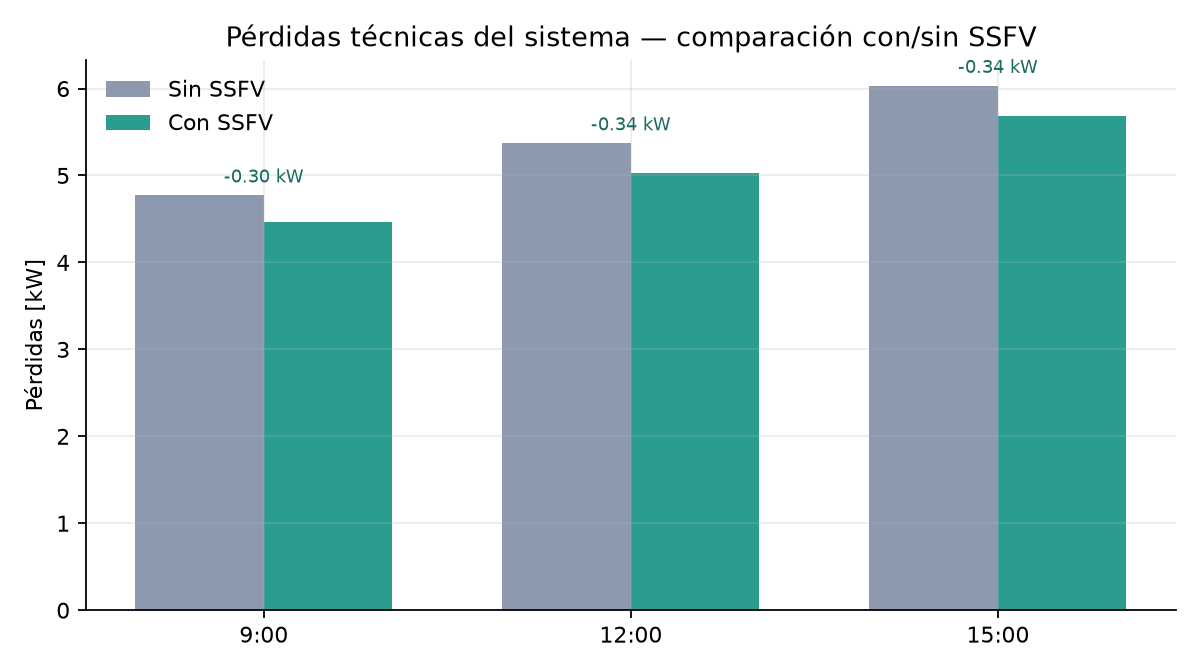
\includegraphics[width=0.90\textwidth]{figuras/fig_perdidas.png}
    \caption{Pérdidas técnicas del sistema con y sin SSFV}
    \label{fig:perdidas}
\end{figure}

\begin{table}[H]
    \centering
    \caption{Pérdidas totales del sistema}
    \begin{tabular}{lccc}
    \toprule
    \textbf{Hora} & \textbf{Con SSFV (kW)} & \textbf{Sin SSFV (kW)} & \textbf{Reducción (kW)} \\
    \midrule
    9:00 a.m. & 4,47 & 4,77 & 0,30 \\
    12:00 p.m. & 5,03 & 5,37 & 0,34 \\
    15:00 & 5,69 & 6,03 & 0,34 \\
    \bottomrule
    \end{tabular}
\end{table}

\textbf{Conclusión:} La generación distribuida reduce las pérdidas técnicas del alimentador en las tres franjas evaluadas.

\subsection{Pérdidas Consideradas en Energía Generada}

\begin{table}[H]
    \centering
    \caption{Desglose de pérdidas del sistema fotovoltaico}
    \begin{tabular}{lc}
    \toprule
    \textbf{Tipo de pérdida} & \textbf{Porcentaje} \\
    \midrule
    Pérdidas por temperatura & 3,00\% \\
    Pérdidas por mismatch & 2,00\% \\
    Pérdidas resistivas & 4,00\% \\
    Pérdidas por conversión DC/AC & 1,00\% \\
    Otras pérdidas asociadas & 16,00\% \\
    Pérdidas por sombreado & 0,00\% \\
    \midrule
    \textbf{Total} & \textbf{26,00\%} \\
    \bottomrule
    \end{tabular}
\end{table}
